\documentclass[conference]{IEEEtran}
\IEEEoverridecommandlockouts
% The preceding line is only needed to identify funding in the first footnote. If that is unneeded, please comment it out.
\usepackage{cite}
\usepackage{amsmath,amssymb,amsfonts}
\usepackage{algorithmic}
\usepackage{graphicx}
\usepackage{textcomp}
\usepackage{amssymb}
\usepackage{float} % for H placement option
\usepackage{listings}
\usepackage[colorlinks=true, linkcolor=red, urlcolor=blue, citecolor=blue]{hyperref}
\usepackage{minted}
\usepackage{xcolor}
\def\BibTeX{{\rm B\kern-.05em{\sc i\kern-.025em b}\kern-.08em
    T\kern-.1667em\lower.7ex\hbox{E}\kern-.125emX}}
\begin{document}

\title{Hard disk failure data analysis\\}

\author{\IEEEauthorblockN{Luca Falasca}
\IEEEauthorblockA{\textit{0334722} \\
luca.falasca@students.uniroma2.eu
}
\and
\IEEEauthorblockN{Matteo Conti}
\IEEEauthorblockA{\textit{0323728} \\
matteo.conti97@students.uniroma2.eu
}\\
}


\maketitle
\thispagestyle{plain}
\pagestyle{plain}

\begin{abstract}
    Questo studio presenta l'implementazione di una pipeline per lo stream processing di dati di grandi dimensioni, finalizzata all'analisi dei fallimenti dei dischi rigidi. La pipeline, containerizzata e gestita tramite Docker Compose, utilizza Apache Kafka per l'ingestion dei dati e la pubblicazione dell'output del processamento ed Apache Flink per il processamento. Il dataset analizzato, una versione ridotta di quello del Grand Challenge della conferenza ACM DEBS 2024, contiene informazioni su data di misurazione, identificativo del disco rigido, modello, ore di accensione e fallimenti. Per analizzare i dati e confrontare le prestazioni dei formati di file CSV e Parquet sono state eseguite tre query. TODO
\end{abstract}

\section{Introduzione}
\subsection{Descrizione del problema}
Il problema da affrontare consiste nell'eseguire stream processing di un dataset mediante l'uso di una pipeline basata su framework per Big Data simulando l'arrivo in real time dei dati. Nello specifico, l'obiettivo è analizzare un dataset contenente informazioni relative ai fallimenti dei dischi rigidi attraverso l'esecuzione di 3 query.
\subsection{Obiettivi}
L'obbiettivo del progetto è quello di eseguire le query proposte su Apache Flink e di valutare le prestazioni ottenute dalle stesse in termini di latenza e througput.
\subsection{Dataset}
Il dataset fornito è una versione ridotta di quello presentato nel Grand Challenge della conferenza ACM DEBS 2024. Delle numerose colonne presenti nel dataset, ne verranno selezionate solamente sette per l'esecuzione delle query, in particolare:
\begin{itemize}
    \item \textit{date}: data della misurazione
    \item \textit{serial\_number}: identificativo del disco rigido
    \item \textit{failure}: indica se il disco rigido ha avuto una failure o meno
    \item \textit{model}: modello del disco rigido
    \item \textit{vault\_id}: identificativo del gruppo di storage server
    \item \textit{s9\_power\_on\_hours}: ore di accensione del disco rigido
    \item \textit{s194\_temperature\_celsius}: temperatura del disco rigido in gradi celsius
\end{itemize}
Esplorando il dataset si può notare un'ambiguità nella colonna \textit{s9\_power\_on\_hours}, essa contiene dei valori 0. Questi valori possono essere interpretati in due modi:
\begin{itemize}
    \item Il dato è un errore di misurazione e quindi va eliminato
    \item Il disco rigido è stato acceso per meno di un'ora al momento della misurazione
\end{itemize}
Date le seguenti considerazioni si è deciso di non eliminare i valori 0 e considerarli quindi validi. Questo andrà ad influenzare i risultati della query 3, in particolare questo sarà molto evidente per quanto riguarda il minimo delle ore di accensione.
Le colonne \textit{s9\_power\_on\_hours} e \textit{s194\_temperature\_celsius} contiene anche diversi valori nulli, le righe corrispondenti a tali valori verranno eliminate in fase di preprocessamento.
Inoltre, righe di header ripetute ad esempio righe in cui il campo \textit{vault\_id} non è un intero bensì la stringa "vault\_id", anche questa volta tali righe verranno eliminate in fase di preprocessamento.

\section{Pipeline}
Per la gestione dei dati relativi ai guasti dei dischi rigidi, è stata implementata una pipeline (Fig. \ref{fig:pipeline}) il cui deploy è stato fatto tramite Docker Compose. La pipeline è composta da diverse componenti, ognuna delle quali svolge un compito specifico, in particolare è stato utilizzato Apache Kafka come sistema publish subscriber per la data ingestion e la scrittura dell'output ed Apache Flink per lo stream processing. Di seguito verrano illustrati i dettagli di ciascuna componente.
\begin{figure}[H]
    \centering
    
\includegraphics[width=0.5\textwidth]{./res/pipeline.png}
    \caption{Pipeline ad alto livello}
    \label{fig:pipeline}
\end{figure} 

\subsection{Data Ingestion}
Per quanto riguarda la data ingestion è stato sviluppato un programma che simula il replay del dataset in maniera accelerata. Il replay viene accelerato di un fattore 3600, in modo tale che ogni secondo di tempo reale corrisponda ad un'ora di tempo simulato. Tuttavia dato che il dataset contiene delle tuple a granularità di giornaliera, per evitare di inviare i dati a burst ogni giorno, i dati della giornata vengono spalmati uniformemente all'interno di essa. Per farlo ogni giornata è stata logicamente divisa in 150000 parti, un numero che è stato scelto appositamente maggiore del numero di tuple presenti in ogni giornata, e ad ogni parte che dura 1/150000 di giorno corrisponde un invio di una tupla al sistema. Per fare in modo che il tempo sia scandito nel modo corretto, viene calcolato a priori il tempo relativo all'invio della prima tupla e poi viene misurato quando effettivamente viene mandata, a quel punto si fa una sleep del tempo rimanente a riempire lo slot. Inoltre, dato che le tuple non sono esattamente 150000 per ogni giornata, gli slot non vengono riempiti mai tutti, e quindi alla fine della giornata si fa una sleep per riempire il tempo rimanente fino a 1 giorno. L'invio dei dati viene fatto in kafka su un topic dedicato che poi sarà consumato da flink.
\subsection{Data Stream Processing}
Per il processamento streaming dei dati, e quindi l'esecuzione delle query, è stato utilizzato il framework Apache Flink, in particolare utilizzando la libreria PyFlink. È stato utilizzato un cluster composto da uno job manager ed un task manager dotato di un task slot (Fig. \ref{fig:flink_cluster}).
Flink consuma i dati da Kafka, filtrati, processati e successivamente pubblicati nuovamente in un topic Kafka. Per effettuare le query sono state utilizzate le API dei Datastream. 
\begin{figure}[H]
    \centering
    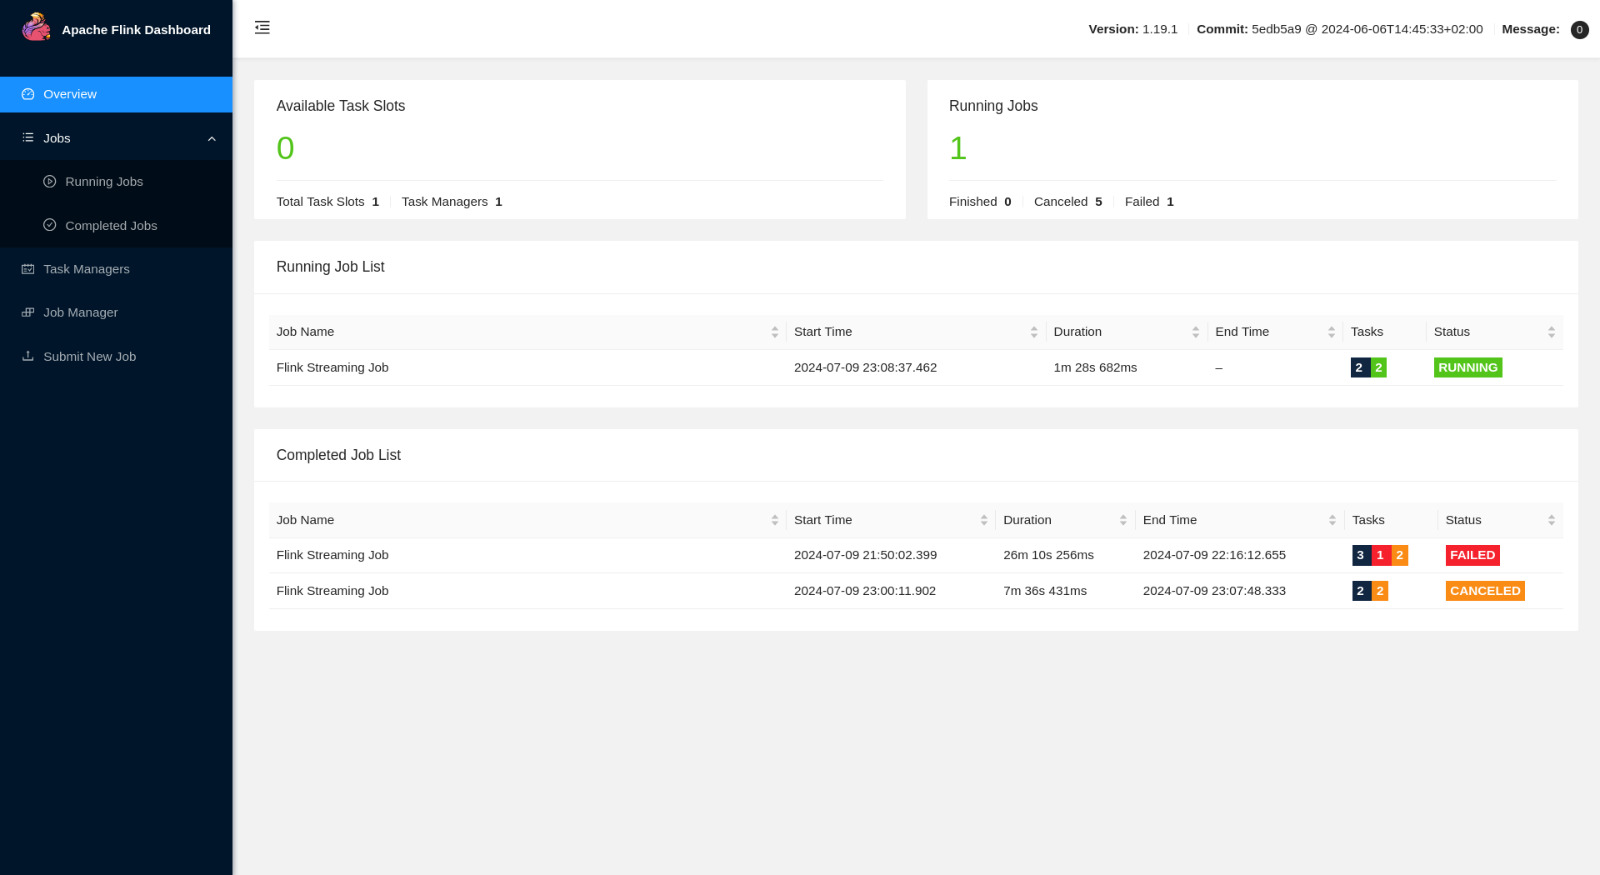
\includegraphics[width=0.5\textwidth]{./res/flink_cluster.jpeg}
    \caption{Cluster Flink}
    \label{fig:flink_cluster}
\end{figure} 

\subsubsection{Query 1}
La prima query prevede di calcolare, per i vault (campo \textit{vault\_id}) con identificativo compreso tra 1000 e 1020,  il numero di eventi valutati, il valor medio e la deviazione standard della temperatura misurata sui suoi hard disk (campo s194\_temperature\_celsius). Per prima cosa vengono generate la source ed il sink Kafka e successivamente, tramite una map, dalle tuple in ingresso vengono estratte le colonne di interesse nel caso di righe del dataset valide e vengono generate delle tuple \textit{Invalid CSV line} per le righe del dataset non valide, al passo successivo tali tuple vengono filtrate. Dopo la fase di filtraggio viene definito come vengono generati i watermark e le tuple vengono marchiate con un timestamp basato sul campo \textit{date} convertito in millisecondi, ricevuto il timestamp vengono filtrate le tuple con \textit{vault\_id} compreso tra 1000 e 1020.
Sulle rimanenti tuple viene fatto keyBy sul campo \textit{vault\_id} considerando finestra di un giorno, tre giorni o globale (chiusa tramite trigger basato sul process time) a seconda della configurazione; le tuple nella finestra vengono aggregate utilizzando una funzione che si occupa di calcolare il numero di eventi valutati, il valor medio e la varianza della temperatura misurata sui suoi hard disk. Infine al risultato viene applicata una map per convertire la varianza in deviazione standard e successivamente viene scritto nel topic Kafka di output relativo alla prima query. Il calcolo avviene tramite una realizzazione di \textit{AggregateFunction} la quale permette di definire un accumulatore i cui campi possono essere aggiornati ad ogni tupla in arrivo, nel nostro caso l'accumulatore è composto da 5 campi cioè la data della prima tupla relativa ad un certo vault id ricevuta, il vault id della tupla corrente, un contatore che aumenta di 1 ad ogni tupla ricevuta, e due campi che si occupano di implementare \textit{l'algoritmo di Welford}\cite{b1} per il calcolo online di media e varianza.
In particolare per il calcolo di media e varianza sono state utilizzate le seguenti relazioni:
\begin{equation}
    \begin{aligned}
        \overline{x}_{k+1} &= \overline{x}_k + \frac{x_{k+1} - \overline{x}_k}{k+1} \\
        \sigma^2_{k+1} &= \sigma^2_k + \frac{(x_{k+1} - \overline{x}_k)(x_{k+1} - \overline{x}_{k+1})}{k+1}
    \end{aligned}
\end{equation}

\subsubsection{Query 2}
La seconda query prevede di calcolare la classifica aggiornata in tempo reale dei 10 vault che registrano il più alto numero di fallimenti nella stessa giornata. Per ogni vault va riportato il numero di fallimenti ed il modello e numero seriale degli hard disk guasti. Per prima cosa vengono generate la source ed il sink Kafka e successivamente, tramite una map, dalle tuple in ingresso vengono estratte le colonne di interesse nel caso di righe del dataset valide e vengono generate delle tuple \textit{Invalid CSV line} per le righe del dataset non valide, al passo successivo tali tuple vengono filtrate. Dopo la fase di filtraggio viene definito come vengono generati i watermark e le tuple vengono marchiate con un timestamp basato sul campo \textit{date} convertito in millisecondi, assegnato il timestamp sulle tuple viene fatto keyBy sul campo \textit{vault\_id} considerando finestra di un giorno, tre giorni o globale (chiusa tramite trigger basato sul process time) a seconda della configurazione. Le tuple nella finestra vengono aggregate tramite un \textit{AggregateFunction} che si occupa, tramite accumulatore, di mantenere la data della prima tupla della finestra e, per ogni vault id, calcolare il numero di fallimenti e mantenere una lista contenente il modello ed il numero seriale degli hard disk guasti. All'output dell'aggregazione viene racchiuso in una finestra con una \textit{window\_all} applicata una \textit{ProcessAllWindowFunction} che si occupa di calcolare la classifica, questo viene fatto ordinando tutte le tuple nella finestra sul campo che riporta il numero di failure e prendendo le prime 10, l'utilizzo di window\_all e della ProcessAllWindowFunction è stata necessaria per poter effettuare l'ordinamento sull'intero contenuto della finestra. Infine il risultato viene scritto nel topic Kafka di output relativo alla seconda query.

\subsubsection{Query 3}
La terza query prevede di calcolare il minimo, 25-esimo, 50-esimo, 75-esimo percentile e massimo delle ore di funzionamento (campo \textit{s9\_power\_on\_hours}) degli hark disk per i vault con identificativo tra 1090 e
1120 (compresi) in real time, senza accumulare tutti i valori. Per prima cosa vengono generate la source ed il sink Kafka e successivamente, tramite una map, dalle tuple in ingresso vengono estratte le colonne di interesse nel caso di righe del dataset valide e vengono generate delle tuple \textit{Invalid CSV line} per le righe del dataset non valide, al passo successivo tali tuple vengono filtrate. Dopo la fase di filtraggio viene definito come vengono generati i watermark e le tuple vengono marchiate con un timestamp basato sul campo \textit{date} convertito in millisecondi, ricevuto il timestamp vengono filtrate le tuple con \textit{vault\_id} compreso tra 1090 e 1120. Sulle rimanenti tuple viene fatto keyBy sul campo \textit{vault\_id} considerando finestra di un giorno, tre giorni o globale (chiusa tramite trigger basato sul process time) a seconda della configurazione; Le tuple nella finestra vengono aggregate tramite un \textit{AggregateFunction} che si occupa, tramite accumulatore, di mantenere la data della prima tupla della finestra e, per ogni vault id, calcolare il minimo, 25-esimo, 50-esimo, 75-esimo percentile e massimo delle ore di funzionamento tramite l'algoritmo \textit{PSquare}\cite{b2}. In particolare ad ogni tupla ricevuta vengono aggiornati gli accumulatori relativi ad i valori del PSquare e vengono confrontati i valori di \textit{s9\_power\_on\_hours} con i valori di min e max precedenti ed aggiornarli se necessario, in questo modo i percentili sono stimati ma mentre il minimo ed il massimo sono esatti pur non mantenendo tutti i valori. Infine il risultato viene scritto nel topic Kafka di output relativo alla terza query.

\subsection{Data Output}
Per la scrittura dell'output del processamento è stato utilizzato Apache Kafka, in particolare sono stati creati tre topic, uno per ogni query, in cui vengono scritti i risultati delle stesse. I topic sono stati creati tramite un'apposita API di Kafka e vengono consumati da un'applicazione esterna che si occupa di scrivere i risultati su file in formato csv

\subsection{Analisi delle prestazioni}
\subsubsection{Metriche}
Le metriche misurate per le 3 query sono la latenza e il throughput. 
\begin{itemize}
    \item Per la latenza è stata utilizzata una metrica custom tramite l'oggetto Gauge offerto da Flink che fornisce metriche on demand
    \item Per il throughput è stata utilizzata la metrica built-in di Flink che fornisce il throughput in elementi al secondo NumRecordsOutPerSecond
\end{itemize}
Entrambe queste metriche sono disponibili tramite l'interfaccia web di Flink e sono accessibili tramite REST API. Quindi le suddette metriche sono state campionate ad intervalli regolari di 1 secondo tramite uno script python che fa richieste alle REST API di Flink e salva i risultati in un file csv per poi graficarli.
\subsubsection{Query 1}
Si può notare che per la prima query i risultati per le finestre di 1 giorno e 3 giorni sono essenzialmente gli stessi, mantenendo una latenza e throughput pressochè costanti. Tuttavia nella finestra globale si può notare un risultato differente in cui il throughput e la latenza aumentano in maniera lineare fino alla fine del processamento. Questo è probabilmente dovuto al fatto che la finestra globale mandando il risultato solo alla fine del processamento non ha throughput limitato dal dover mandare il risultato ad intervalli regolari.
\begin{figure}[H]
    \centering
    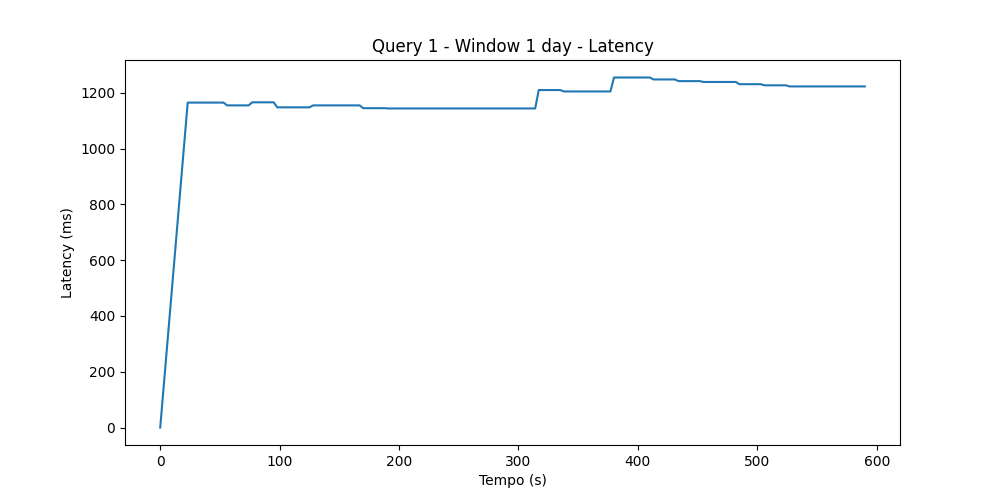
\includegraphics[width=0.5\textwidth]{./res/q1_w1_latency.png}
    \caption{Latency Query 1 - Window 1 day}
    \label{fig:query1_latency_w1}
\end{figure}
\begin{figure}[H]
    \centering
    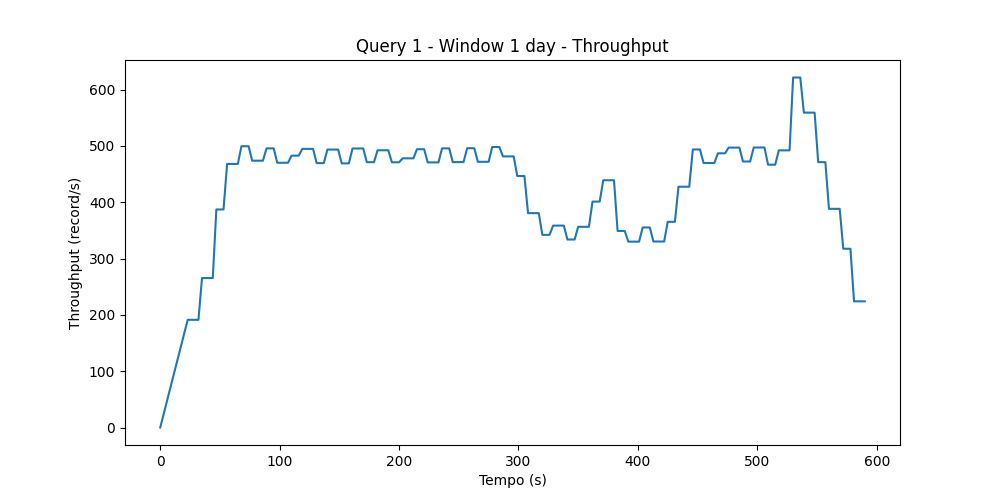
\includegraphics[width=0.5\textwidth]{./res/q1_w1_throughput.png}
    \caption{Throughput Query 1 - Window 1 day}
    \label{fig:query1_throughput_w1}
\end{figure}
\begin{figure}[H]
    \centering
    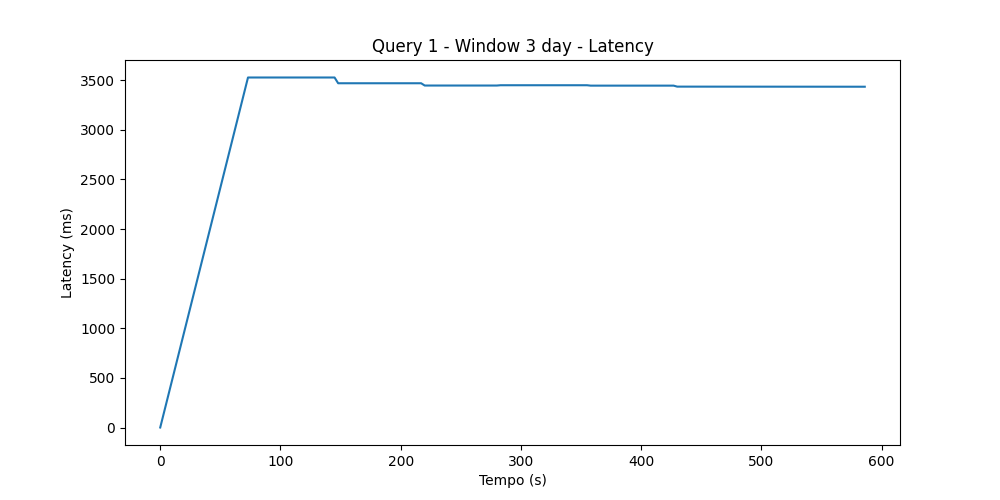
\includegraphics[width=0.5\textwidth]{./res/q1_w2_latency.png}
    \caption{Latency Query 1 - Window 3 day}
    \label{fig:query1_latency_w2}
\end{figure}
\begin{figure}[H]
    \centering
    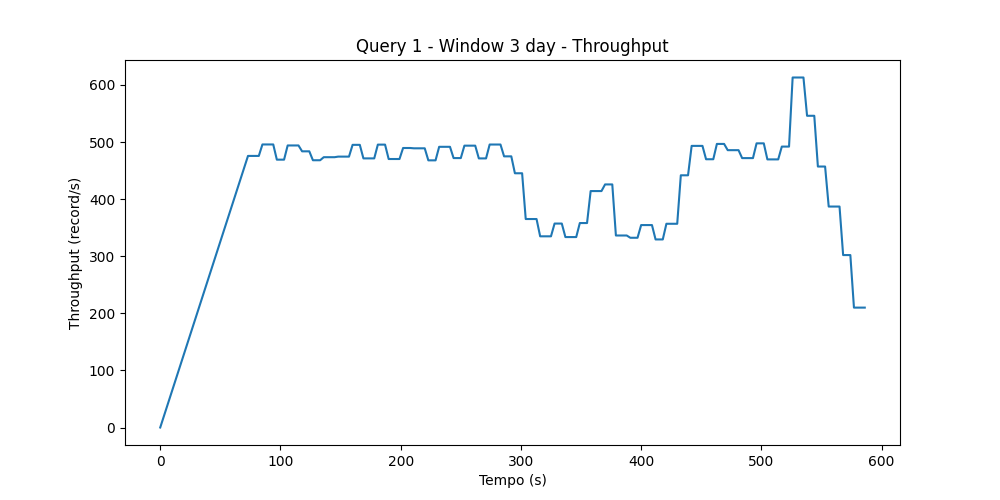
\includegraphics[width=0.5\textwidth]{./res/q1_w2_throughput.png}
    \caption{Throughput Query 1 - Window 3 day}
    \label{fig:query1_throughput_w2}
\end{figure}
\begin{figure}[H]
    \centering
    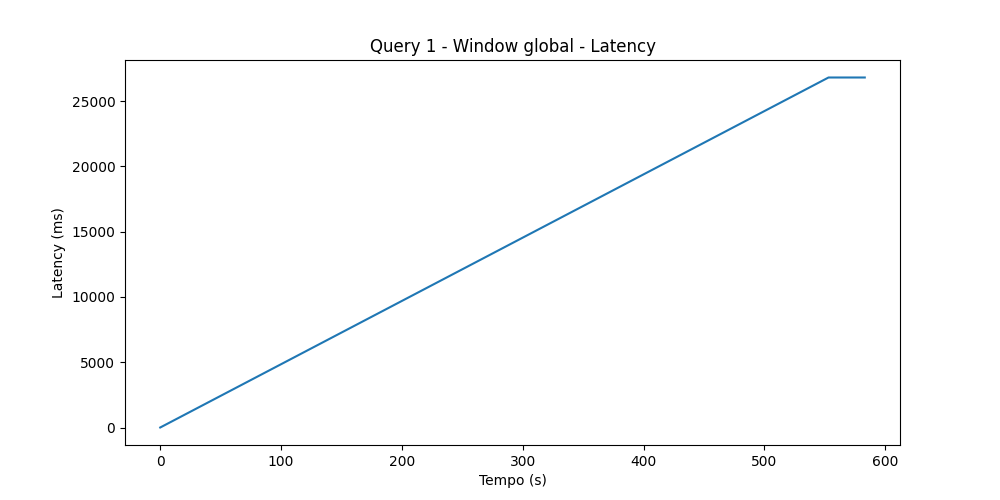
\includegraphics[width=0.5\textwidth]{./res/q1_w3_latency.png}
    \caption{Latency Query 1 - Window Global}
    \label{fig:query1_latency_w3}
\end{figure}
\begin{figure}[H]
    \centering
    
\includegraphics[width=0.5\textwidth]{./res/q1_w3_throughput.png}
    \caption{Throughput Query 1 - Window Global}
    \label{fig:query1_throughput_w3}
\end{figure}
\subsubsection{Query 2}
\subsubsection{Query 3}
\subsubsection{Configurazione ambiente}
\char200{} \\
Risorse hardware
\begin{minted}[autogobble, fontsize=\scriptsize, frame=lines]{text}
    Processors: AMD Ryzen™ 5 7530U with Radeon™ Graphics × 12
    Memory: 16.0 GiB of RAM
    Graphics Processor: AMD Radeon™ Graphics
\end{minted}
Risorse Docker
\begin{minted}[autogobble, fontsize=\scriptsize, frame=lines]{text}
    Processors: 6 core
    Memory: 4 GiB of RAM
\end{minted}
Risorse Flink
\begin{minted}[autogobble, fontsize=\scriptsize, frame=lines]{text}
    Task Managers: 1
    Task Slots: 1
\end{minted}
\subsubsection{Risultati}

\section{Riferimenti}
\begin{itemize}
    \item \href{https://github.com/matteo-conti-97/hard_disk_failure_data_stream_processing}{Codice sorgente github}
\end{itemize}
\begin{thebibliography}{00}
    \bibitem{b1} R. Jain, I. Chlamtac. \href{https://www.cse.wustl.edu/~jain/papers/ftp/psqr.pdf}{"The $P^2$ Algorithm for Dynamic Calculation of Quantiles and Histograms Without Storing Observations."}.
    \bibitem{b2} Welford's algorithm \url{https://en.m.wikipedia.org/wiki/Algorithms_for_calculating_variance\#Welford%27s_online_algorithm}
\end{thebibliography}
\vspace{12pt}
\end{document}

    